\chapter{System Model}
\label{chap:model}

% Put all figures in the directory of ``figure'' in the PDF format. Editable versions of
% the figures with the same filenames as their PDF versions should go into the directory of 
% ``figure\_src'' for easy access.

\section{System Overview}

In this paper, we consider a LEO satellite communication system shown in Figure~\ref{fig_system}. There are $N$ satellites denoted as $\mathcal{N} = \{n \mid n = 1, 2, \ldots, N\}$, and each satellite has $M$ beams denoted as $\mathcal{M} = \{m \mid m = 1, 2, \ldots, M\}$. The coverage area covers $K$ cells on the ground denoted as $\mathcal{K} = \{k \mid k = 1, 2, \ldots, K\}$. There are $U$ user equipments (UEs) in the coverage area denoted as $\mathcal{U} = \{u \mid u = 1, 2, \ldots, U\}$. A hexagonal grid of cells and quasi-earth-fixed cell scheme is considered.

\begin{figure}[h!]
    \centering
    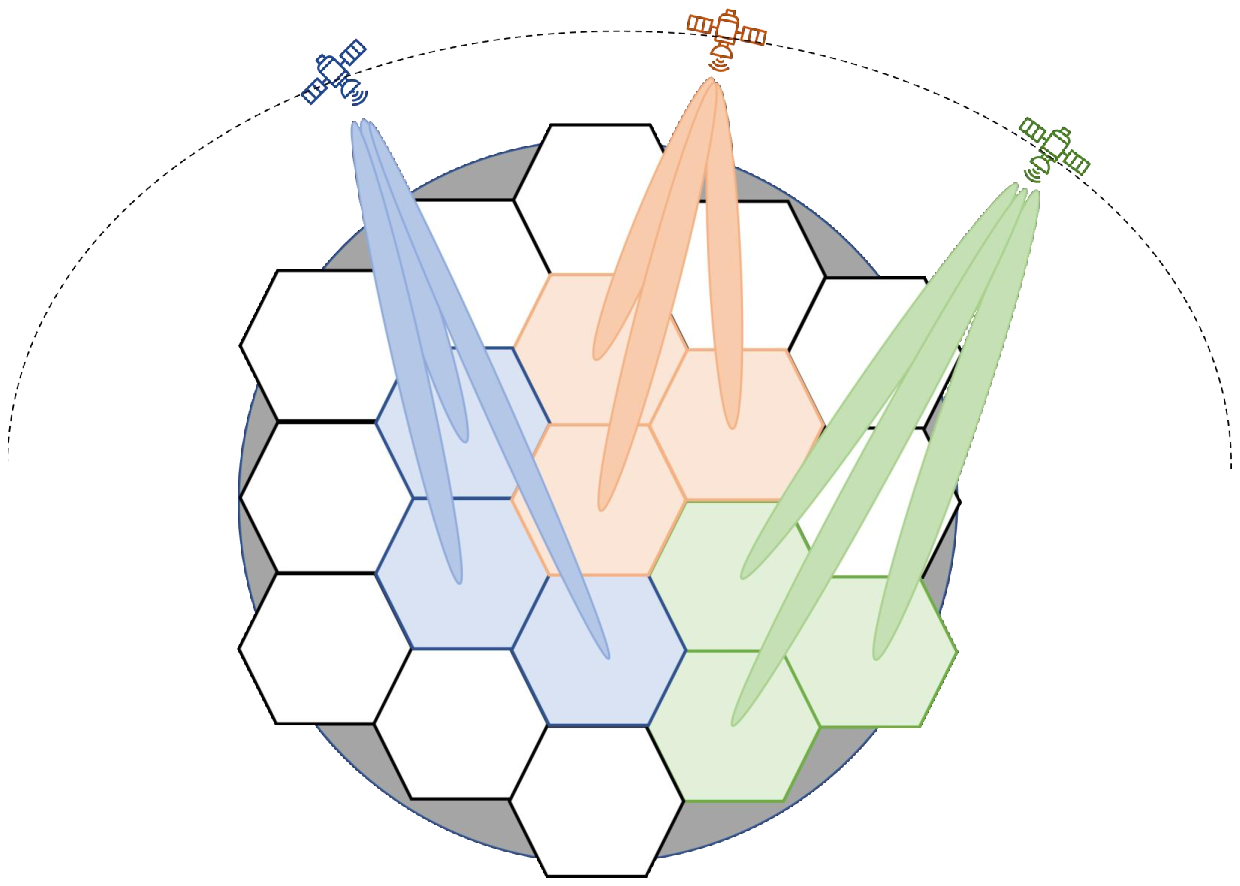
\includegraphics[width=0.8\textwidth]{figure/system overview.pdf}
    \caption{Illustration of satellite beams and cells}
    \label{fig_system}
\end{figure}

\section{Channel Model}

\subsection{Free Space Path Loss}

In the LEO satellite system, the free space path loss from satellite $n$ to cell $k$ can be express as follows~\cite{Satellite-Multi-Beam}:
\begin{equation}
    L_{n,k} = \left(\frac{\lambda}{4\pi d_{n,k}}\right)^2
\end{equation}
where $\lambda$ is the wavelength,and $d$ is the distance between the $n$-th satellite and the center of the $k$-th cell.

\subsection{Shadowed-Rician Fading Channel}

The shadowed-Rician fading model is suitable for satellite communication systems because it accurately reflects the physical propagation environment, capturing both the presence of a strong LoS signal and the effects of shadowing from obstacles~\cite{channel-model}. Let $h_{n,k}$ denote the channel gain between the $n$th satellite and the $k$th cell. The cumulative distribution function (CDF) of the channel gain:
\begin{equation}
F_{h_{n,k}}(x) = K \sum_{n=0}^{\infty} \frac{(m)_n \, \delta^n \, (2b)^{1+n}}{(n!)^2} \, \gamma\left(1+n, \frac{x}{2b}\right)
\end{equation}

where $K = (2bm/(2bm+\Omega))^m/2b$, $\delta = \Omega/(2bm+\Omega)/2b$. $\Omega$ is the average power of LoS component, and $2b$ is the average power of the multi-path component except the LoS component. $m$ is the Nakagami parameter.

% In the LEO satellite system, the free space path loss defined by 3GPP protocol is as follows~\cite{38811}:
% \begin{equation}
% PL = 32.45 + 20\log_{10}(f_c) + 20\log_{10}(d),
% \end{equation}
% where $f_c$ is the carrier frequency and $d$ is the distance between the satellite and its serving cell position.
\subsection{Antenna Radiation Pattern}
We introduce the antenna radiation pattern in~\cite{Energy-Efficient}:
\begin{equation}
G(\theta_{n,m,u}) = G_{max} \left[ \frac{J_1\left(\mu(\theta_{n,m,u})\right)}{2\mu(\theta_{n,m,u})} 
+ 36 \frac{J_3\left(\mu(\theta_{n,m,u})\right)}{\mu(\theta_{n,m,u})^3} \right]^2,
\end{equation}
where $\theta_{n,m,u}$ represents the boresight angle between the user position and the beam center with respect to the satellite, $G_{max}$ is the maximum antenna gain, $\mu(\theta) = 2.07123\cdot \sin(\theta)/\sin(\theta_{3dB})$, 
where $\theta_{3dB}$ is the 3 dB half-power beamwidth angle of the antenna, and $J_1(\cdot)$ and $J_3(\cdot)$ represent the Bessel functions of the first kind of orders 1 and 3.

% And considering the rain fading effect, we introduce a raining fading factor follows the Gaussian distribution $r~\sim \mathcal{N}(\mu, \sigma)$, where $\mu$ and $\sigma$
% depends on the location, polarization, and elevation angle between UE and satellite~\cite{User-Scheduling}. 
% Also, considering the payload (PL) oscillator phase noise $n_{theta}$ at the n-th satellite that follows a Gaussian distribution with zero mean and standard deviation 0.24:
% \begin{equation}
%     \hat\theta_{n,u} = \theta_{n,u} + n_{theta}
% \end{equation}
Thus, with the transmitted power $P_{m,n}$ from the $m$-th beam of the $n$-th satellite, the received power from the $m$-th beam of the $n$-th satellite to the $u$-th user $\hat{P}_{n,m,u}$ can be expressed as:
\begin{equation}
    \hat{P}_{n,m,u} = P_{n,m} \cdot L_{n,k} \cdot h_{n,k} \cdot G(\theta_{n,m,u})% \cdot r_{n,u}
\end{equation}

\section{Synchronization Signal Block Model}

Followed by 3GPP protocol~\cite{38331}, the supported synchronization signal block (SSB) periodicity values are \{20, 40, 80, 160\} miliseconds. Here we define the SSB periodicity of each cell:
\begin{equation}
    T^{SSB}_{k}\in\{20, 40, 80, 160\}, \forall k \in K
\end{equation}
We define the duration of each time slot as 160 ms. To simplify computational complexity, it is assumed that both the positions of the satellites and UEs are fixed within each time slot. Furthermore, the SSB periodicity specification for each cell is considered unchanged throughout the slot.

Let $\Delta_{n,m}[t]$ denote the set of cells served by the $m$-th beam of the $n$-th satellite at time slot $t$. Since the time duration of each slot is 160ms and the SSB periodicity is 20, 40, 80, 160ms, the number of element in $\Delta_{n,m}[t]$ must be 1, 2, 4, or 8, as shown in Figure~\ref{delta}.

\begin{figure}[h!]
    \centering
    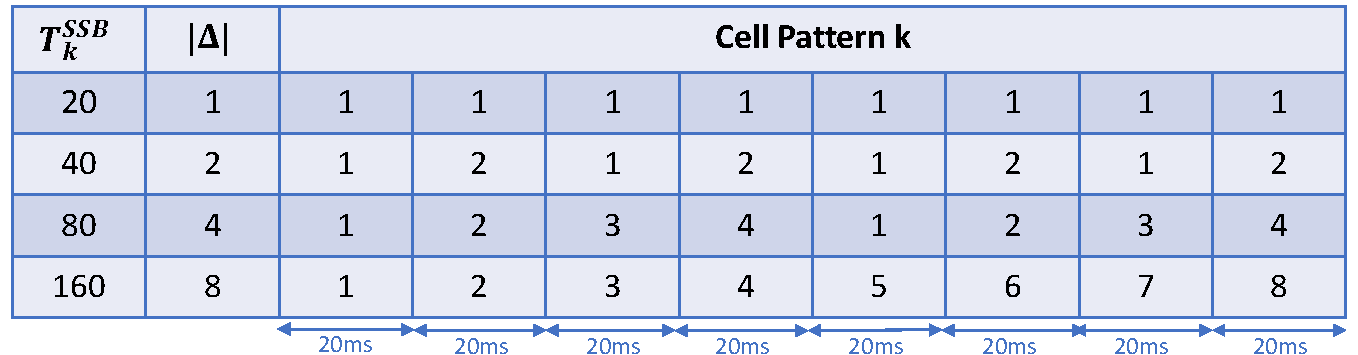
\includegraphics[width=0.8\textwidth]{figure/delta pattern.pdf}
    \caption{Illustration of satellite beams and cells}
    \label{delta}
\end{figure}

\section{UE Random Access Delay}

$T_u$, the $u$-th UE random access delay, is defined as the time duration between the $u$-th UE starts SSB measurement and successfully receives SSB, as shown in Figure~\ref{RAD}. $T_u$ can be further decomposed to two parts, $T_u^i$ and $T_u^l$. $T_u^i$ is defined as the time duration between UE starts SSB measurement and the first SSB arrives. And $T_u^l$ is defined as the time duration between the first SSB arrives to UE succeeds to receive SSB. Since UE can start SSB measurement at any time, $T_u^i$ can be expressed as an uniform distribution random variable $U(0, T_{k_u}^{SSB})$. On the other hand, $T_u^l$ is the multiple of $T_{k_u}^{SSB}$, depending on the number of times the $u$-th UE fails during random access $Q_u$. In this thesis, we define that as long as the UE received SSB power is less than $P_{th}$, the UE will fail to measure SSB. We denote the probability of the received SSB power $\hat{P}_{n, m, u}$ less than $P_{th}$ be $P_u^0$. The mathematical formula can be expressed as follows:
\begin{equation}
    T_u = T_u^i + T_u^l
\end{equation}
\begin{equation}
    F_{T_u^i}(t) = 
    \begin{cases}
        \frac{t}{T_{k_u}^{SSB}}, & 0 \leq t< T_{k_u}^{SSB} \\
        1, & t \geq T_{k_u}^{SSB} \\
        0, & \text{otherwise}
    \end{cases}
\end{equation}
\begin{equation}
    T_u^l = Q_u \cdot T_{k_u}^{SSB}
\end{equation}
\begin{equation}
    \Pr\left[Q_u = n\right] = (1 - P_u^0) (P_u^0)^n
\end{equation}
where $k_u$ is the cell where the $u$-th UE is located.

\begin{figure}[h!]
    \centering
    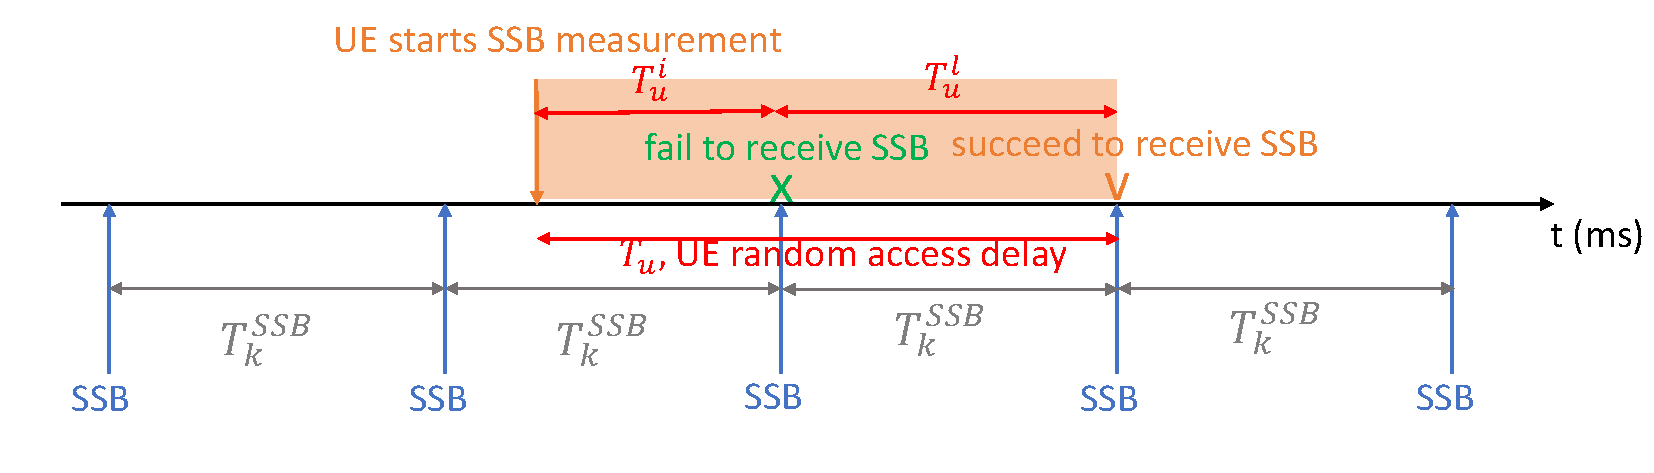
\includegraphics[width=1\textwidth]{figure/random access delay.pdf}
    \caption{Illustration of UE random access delay}
    \label{RAD}
\end{figure}

% $P_{th}$ is the threshold energy that for the received signal energy $P \geq P_th$, UE is able to receive the SSB message successfully.
% $F(t) = \Pr\{T \leq t\}$ is the CDF of user transmission delay.
% We denote $P_{n,m}$ as the transmitted power of $n$-th satellite's $m$-th beam. Due to the power budget, each satellite has a fixed total power $P_s$, that is:
% \begin{equation}
%     P_s = \sum_m P_{n,m}, \forall n \in N
% \end{equation}

\section{Problem Formulation}

During the latest 3GPP meeting, the adjustment and implementation of SSB periodicity in the NGSO scenario were discussed intensively. In the 3GPP RAN1 \#116 meeting \cite{ran1-116}, further specifications for the LEO satellite communication scenario were defined. This raises an important issue: How can satellites provide random access to such a large number of cells with limited power? It is clear that if we extend the SSB periodicity for some cells, the satellites' power consumption is reduced, while the UE random access delay increases. The transmitted power of the SSB also affects the success probability of the random access procedure between satellites and UEs. Thus, this thesis will investigate the trade-off between power allocation, SSB periodicity, and UE random access delay, which can be described by the following mathematical model:

\begin{equation}
\begin{aligned}
    & \underset{\Delta, P_{n, m}}{\text{min}} \sum_{U} T_u \\
    & \text{subject to} \\
    & \qquad \sum_{m} P_{n,m}[t] \leq P_s, \quad \forall n \in \mathbb{N} \\
    & \qquad \Delta_{n, m}[t] \in \{0, 1, 2, 4, 8\}, \quad \forall n \in \mathbb{N}, m \in \mathbb{N} \\
    & \qquad \Delta_{n, m}[t] \cap \Delta_{n', m'}[t] = \emptyset, \quad \forall n, n' \in \{1, 2, \ldots, N\}, m, m' \in \{1, 2, \ldots, M\}, (n, m) \neq (n', m')
\end{aligned}
\end{equation}

where $P_s$ is the maximum transmitted power for each satellite.